\documentclass[10pt]{article}
%DIF LATEXDIFF DIFFERENCE FILE
%DIF DEL old_supplement.tex   Thu Mar 26 19:56:32 2026
%DIF ADD supplement.tex       Thu Mar 26 22:51:30 2026
\usepackage[utf8]{inputenc}
\usepackage[english]{babel}
\usepackage[font=small,labelfont=bf]{caption}
\usepackage{geometry}
\usepackage{natbib}
\usepackage{pxfonts}
\usepackage{graphicx}
\usepackage{newfloat}
\usepackage{setspace}
\usepackage{hyperref}
\usepackage{placeins}
%DIF 13a13-14
\usepackage{float} %DIF > 
\usepackage{caption} %DIF > 
%DIF -------
\usepackage{booktabs}
\usepackage{longtable}

\newcommand{\argmax}{\mathop{\mathrm{argmax}}\limits}
\newcommand{\argmin}{\mathop{\mathrm{argmin}}\limits}

\title{\textit{Supplementary materials for}: A Stylometric Application of Large Language Models}

\author{Harrison F. Stropkay, Jiayi Chen, Mohammad J. Latifi,\\
Daniel N. Rockmore, and Jeremy R. Manning\\
Dartmouth College \\
Hanover, NH 03755, USA \\
\texttt{\{harrison.f.stropkay.25, jiayi.chen.gr, mohammad.javad.latifi.jebelli}\\\texttt{daniel.n.rockmore, jeremy.r.manning\}@dartmouth.edu}}

\date{}
%DIF PREAMBLE EXTENSION ADDED BY LATEXDIFF
%DIF UNDERLINE PREAMBLE %DIF PREAMBLE
\RequirePackage[normalem]{ulem} %DIF PREAMBLE
\RequirePackage{color}\definecolor{RED}{rgb}{1,0,0}\definecolor{BLUE}{rgb}{0,0,1} %DIF PREAMBLE
\providecommand{\DIFaddtex}[1]{{\protect\color{blue}\uwave{#1}}} %DIF PREAMBLE
\providecommand{\DIFdeltex}[1]{{\protect\color{red}\sout{#1}}} %DIF PREAMBLE
%DIF SAFE PREAMBLE %DIF PREAMBLE
\providecommand{\DIFaddbegin}{} %DIF PREAMBLE
\providecommand{\DIFaddend}{} %DIF PREAMBLE
\providecommand{\DIFdelbegin}{} %DIF PREAMBLE
\providecommand{\DIFdelend}{} %DIF PREAMBLE
\providecommand{\DIFmodbegin}{} %DIF PREAMBLE
\providecommand{\DIFmodend}{} %DIF PREAMBLE
%DIF FLOATSAFE PREAMBLE %DIF PREAMBLE
\providecommand{\DIFaddFL}[1]{\DIFadd{#1}} %DIF PREAMBLE
\providecommand{\DIFdelFL}[1]{\DIFdel{#1}} %DIF PREAMBLE
\providecommand{\DIFaddbeginFL}{} %DIF PREAMBLE
\providecommand{\DIFaddendFL}{} %DIF PREAMBLE
\providecommand{\DIFdelbeginFL}{} %DIF PREAMBLE
\providecommand{\DIFdelendFL}{} %DIF PREAMBLE
%DIF HYPERREF PREAMBLE %DIF PREAMBLE
\providecommand{\DIFadd}[1]{\texorpdfstring{\DIFaddtex{#1}}{#1}} %DIF PREAMBLE
\providecommand{\DIFdel}[1]{\texorpdfstring{\DIFdeltex{#1}}{}} %DIF PREAMBLE
\newcommand{\DIFscaledelfig}{0.5}
%DIF HIGHLIGHTGRAPHICS PREAMBLE %DIF PREAMBLE
\RequirePackage{settobox} %DIF PREAMBLE
\RequirePackage{letltxmacro} %DIF PREAMBLE
\newsavebox{\DIFdelgraphicsbox} %DIF PREAMBLE
\newlength{\DIFdelgraphicswidth} %DIF PREAMBLE
\newlength{\DIFdelgraphicsheight} %DIF PREAMBLE
% store original definition of \includegraphics %DIF PREAMBLE
\LetLtxMacro{\DIFOincludegraphics}{\includegraphics} %DIF PREAMBLE
\newcommand{\DIFaddincludegraphics}[2][]{{\color{blue}\fbox{\DIFOincludegraphics[#1]{#2}}}} %DIF PREAMBLE
\newcommand{\DIFdelincludegraphics}[2][]{% %DIF PREAMBLE
\sbox{\DIFdelgraphicsbox}{\DIFOincludegraphics[#1]{#2}}% %DIF PREAMBLE
\settoboxwidth{\DIFdelgraphicswidth}{\DIFdelgraphicsbox} %DIF PREAMBLE
\settoboxtotalheight{\DIFdelgraphicsheight}{\DIFdelgraphicsbox} %DIF PREAMBLE
\scalebox{\DIFscaledelfig}{% %DIF PREAMBLE
\parbox[b]{\DIFdelgraphicswidth}{\usebox{\DIFdelgraphicsbox}\\[-\baselineskip] \rule{\DIFdelgraphicswidth}{0em}}\llap{\resizebox{\DIFdelgraphicswidth}{\DIFdelgraphicsheight}{% %DIF PREAMBLE
\setlength{\unitlength}{\DIFdelgraphicswidth}% %DIF PREAMBLE
\begin{picture}(1,1)% %DIF PREAMBLE
\thicklines\linethickness{2pt} %DIF PREAMBLE
{\color[rgb]{1,0,0}\put(0,0){\framebox(1,1){}}}% %DIF PREAMBLE
{\color[rgb]{1,0,0}\put(0,0){\line( 1,1){1}}}% %DIF PREAMBLE
{\color[rgb]{1,0,0}\put(0,1){\line(1,-1){1}}}% %DIF PREAMBLE
\end{picture}% %DIF PREAMBLE
}\hspace*{3pt}}} %DIF PREAMBLE
} %DIF PREAMBLE
\LetLtxMacro{\DIFOaddbegin}{\DIFaddbegin} %DIF PREAMBLE
\LetLtxMacro{\DIFOaddend}{\DIFaddend} %DIF PREAMBLE
\LetLtxMacro{\DIFOdelbegin}{\DIFdelbegin} %DIF PREAMBLE
\LetLtxMacro{\DIFOdelend}{\DIFdelend} %DIF PREAMBLE
\DeclareRobustCommand{\DIFaddbegin}{\DIFOaddbegin \let\includegraphics\DIFaddincludegraphics} %DIF PREAMBLE
\DeclareRobustCommand{\DIFaddend}{\DIFOaddend \let\includegraphics\DIFOincludegraphics} %DIF PREAMBLE
\DeclareRobustCommand{\DIFdelbegin}{\DIFOdelbegin \let\includegraphics\DIFdelincludegraphics} %DIF PREAMBLE
\DeclareRobustCommand{\DIFdelend}{\DIFOaddend \let\includegraphics\DIFOincludegraphics} %DIF PREAMBLE
\LetLtxMacro{\DIFOaddbeginFL}{\DIFaddbeginFL} %DIF PREAMBLE
\LetLtxMacro{\DIFOaddendFL}{\DIFaddendFL} %DIF PREAMBLE
\LetLtxMacro{\DIFOdelbeginFL}{\DIFdelbeginFL} %DIF PREAMBLE
\LetLtxMacro{\DIFOdelendFL}{\DIFdelendFL} %DIF PREAMBLE
\DeclareRobustCommand{\DIFaddbeginFL}{\DIFOaddbeginFL \let\includegraphics\DIFaddincludegraphics} %DIF PREAMBLE
\DeclareRobustCommand{\DIFaddendFL}{\DIFOaddendFL \let\includegraphics\DIFOincludegraphics} %DIF PREAMBLE
\DeclareRobustCommand{\DIFdelbeginFL}{\DIFOdelbeginFL \let\includegraphics\DIFdelincludegraphics} %DIF PREAMBLE
\DeclareRobustCommand{\DIFdelendFL}{\DIFOaddendFL \let\includegraphics\DIFOincludegraphics} %DIF PREAMBLE
%DIF COLORLISTINGS PREAMBLE %DIF PREAMBLE
\RequirePackage{listings} %DIF PREAMBLE
\RequirePackage{color} %DIF PREAMBLE
\lstdefinelanguage{DIFcode}{ %DIF PREAMBLE
%DIF DIFCODE_UNDERLINE %DIF PREAMBLE
  moredelim=[il][\color{red}\sout]{\%DIF\ <\ }, %DIF PREAMBLE
  moredelim=[il][\color{blue}\uwave]{\%DIF\ >\ } %DIF PREAMBLE
} %DIF PREAMBLE
\lstdefinestyle{DIFverbatimstyle}{ %DIF PREAMBLE
	language=DIFcode, %DIF PREAMBLE
	basicstyle=\ttfamily, %DIF PREAMBLE
	columns=fullflexible, %DIF PREAMBLE
	keepspaces=true %DIF PREAMBLE
} %DIF PREAMBLE
\lstnewenvironment{DIFverbatim}{\lstset{style=DIFverbatimstyle}}{} %DIF PREAMBLE
\lstnewenvironment{DIFverbatim*}{\lstset{style=DIFverbatimstyle,showspaces=true}}{} %DIF PREAMBLE
\lstset{extendedchars=\true,inputencoding=utf8}

%DIF END PREAMBLE EXTENSION ADDED BY LATEXDIFF

\begin{document}

\renewcommand{\figurename}{Supplementary Figure}
\renewcommand{\tablename}{Supplementary Table}

\newcommand{\crossentropy}{{1}}
\newcommand{\ttests}{{2}}
\newcommand{\confusion}{{3}}
\newcommand{\mds}{{4}}

\newcommand{\authortable}{{1}}


\setcounter{equation}{0}
\setcounter{figure}{0}
\setcounter{table}{0}
\setcounter{page}{1}
\setcounter{section}{0}
\makeatletter


\begin{titlepage}
\maketitle
\end{titlepage}

\begin{figure*}[h]
  \centering
  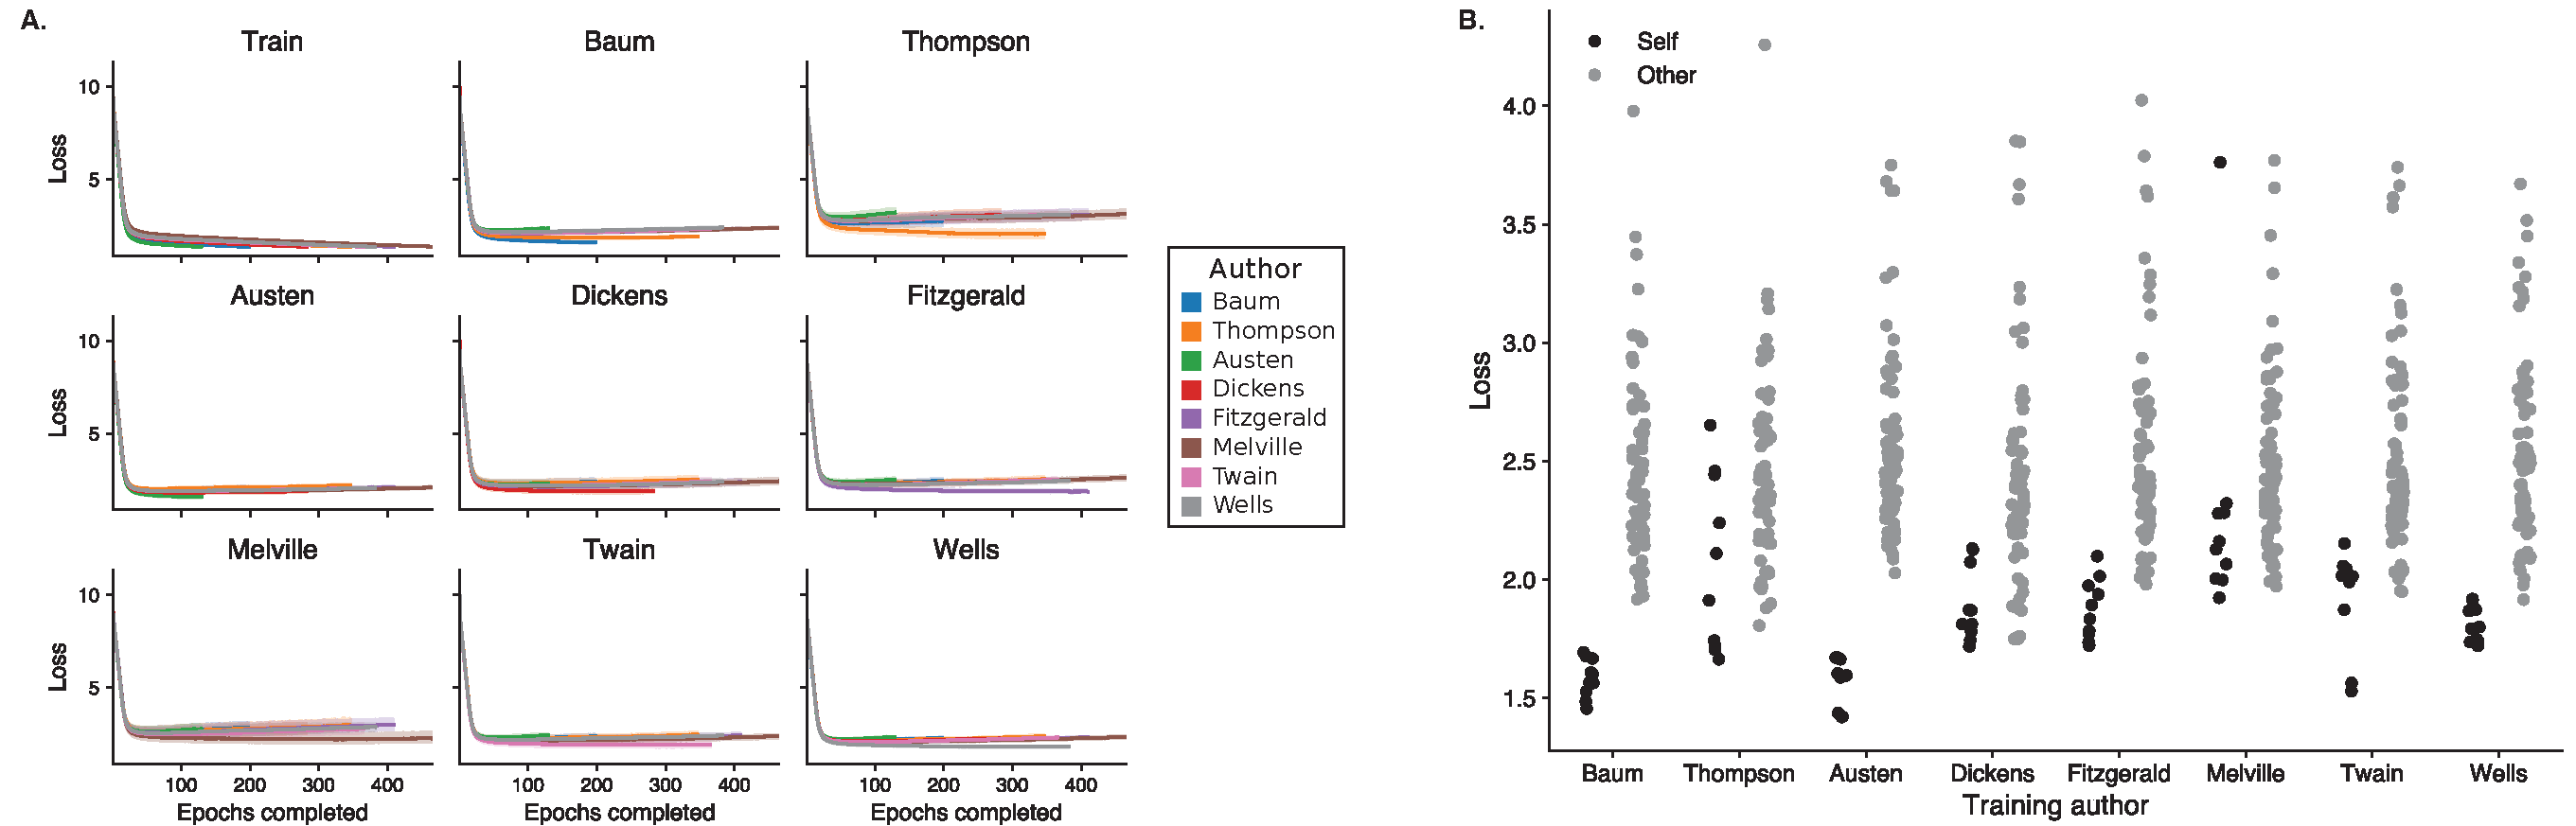
\includegraphics[width=\textwidth]{figs/loss_all_authors_content_only.pdf}


  \caption{\textbf{Cross-entropy loss across models and
      authors using only content words.} Follows the general format of Figure~\crossentropy~in the main text,
      but uses models trained on only content words. All function words are masked out using \texttt{<FUNC>}.
      \textbf{A.} Average cross-entropy loss on
    \textit{Train}ing data and held-out test data from each author,
    plotted as a function of the number of training epochs. Each color
    denotes a model trained on a single author's work.  Error ribbons
    denote bootstrap-estimated 95\% confidence intervals over 10
    random seeds. \textbf{B.} Cross-entropy loss assigned to held-out
    test data by each author's model ($x$-axis). Held-out test data is
    either from the \textit{same} author (black) or from
    \textit{other} authors (gray). Each dot denotes the average loss
    (across all 1024-token chunks) for a single random seed.}
\label{fig:all-losses-content}
\end{figure*}

\begin{figure*}[h]
  \centering
  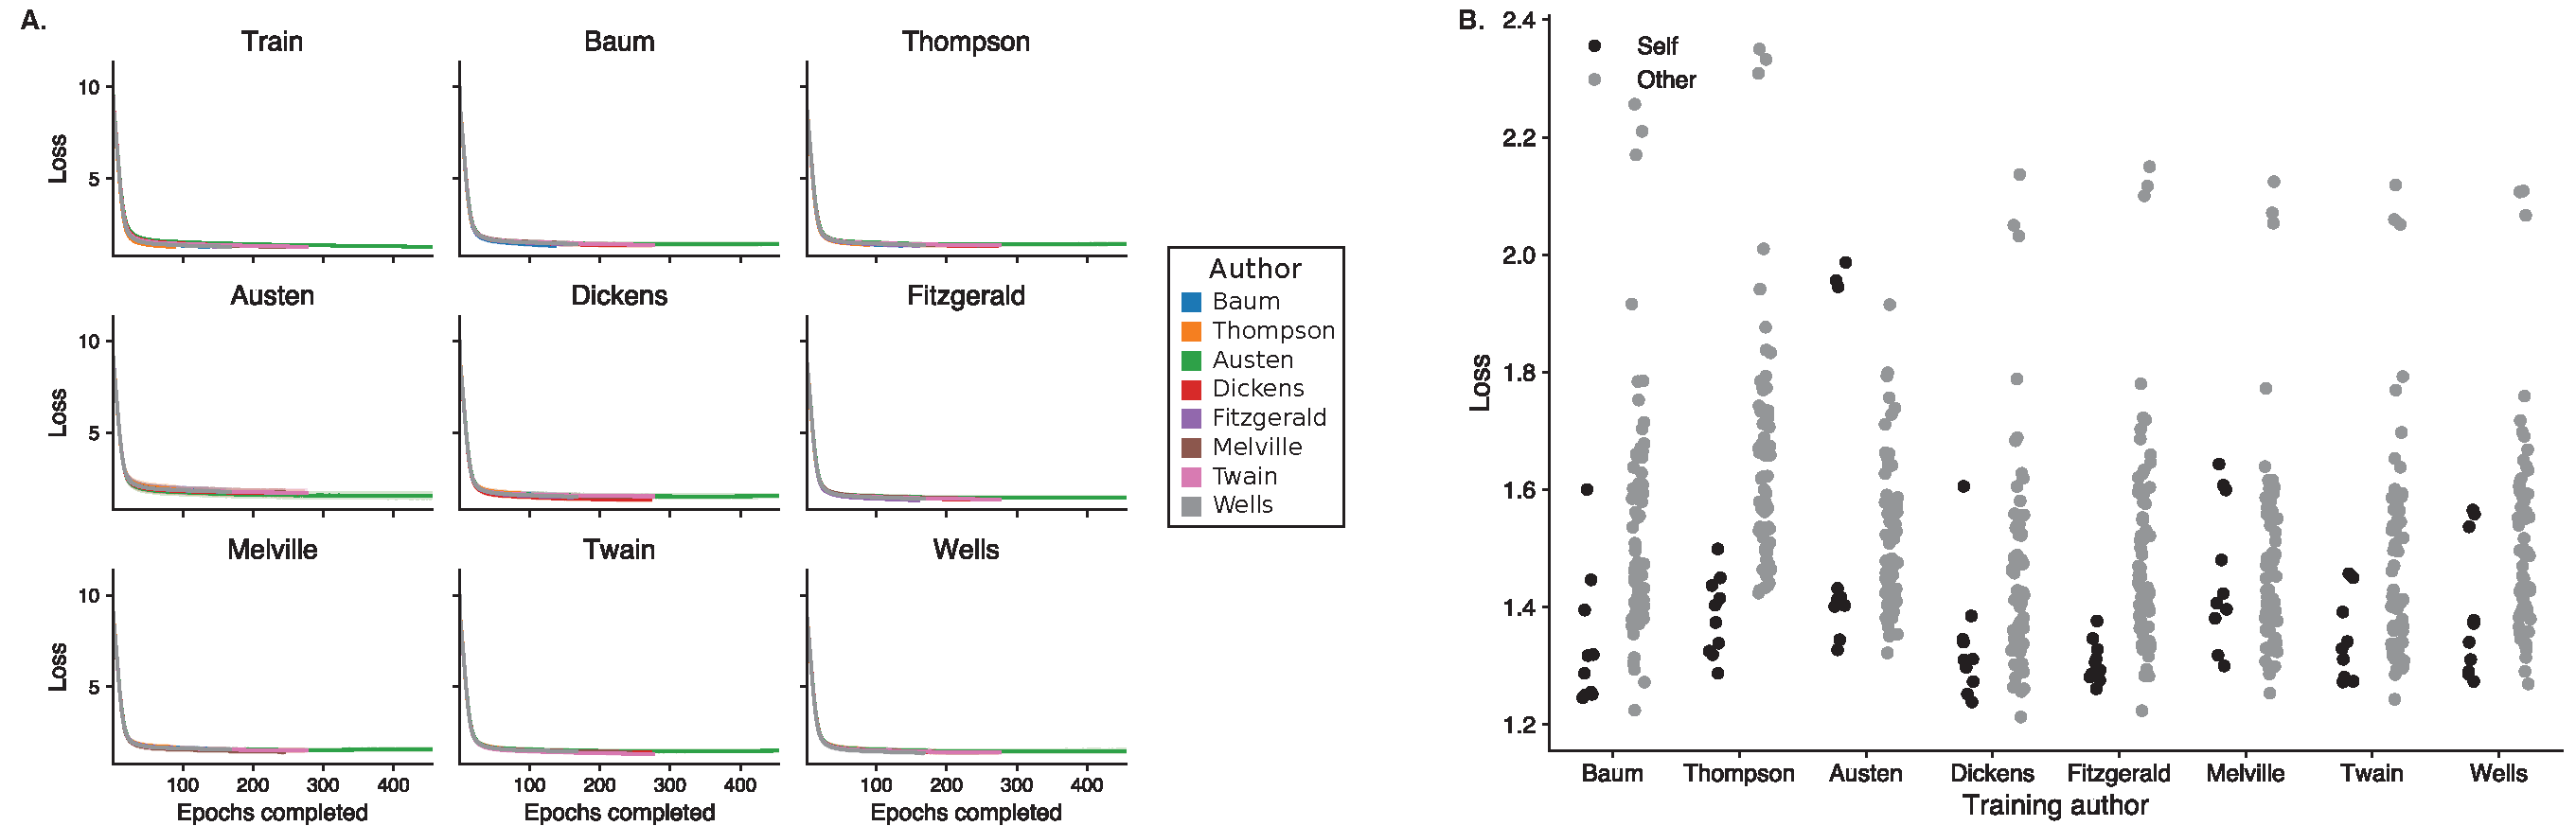
\includegraphics[width=\textwidth]{figs/loss_all_authors_function_only.pdf}


  \caption{\textbf{Cross-entropy loss across models and
      authors using only function words.} Follows the general format of Figure~\crossentropy~in the main text,
      but uses models trained on only function words. All content words are masked out using \texttt{<CONTENT>}.
      \textbf{A.} Average cross-entropy loss on
    \textit{Train}ing data and held-out test data from each author,
    plotted as a function of the number of training epochs. Each color
    denotes a model trained on a single author's work.  Error ribbons
    denote bootstrap-estimated 95\% confidence intervals over 10
    random seeds. \textbf{B.} Cross-entropy loss assigned to held-out
    test data by each author's model ($x$-axis). Held-out test data is
    either from the \textit{same} author (black) or from
    \textit{other} authors (gray). Each dot denotes the average loss
    (across all 1024-token chunks) for a single random seed.}
\label{fig:all-losses-function}
\end{figure*}

\begin{figure*}[h]
  \centering
  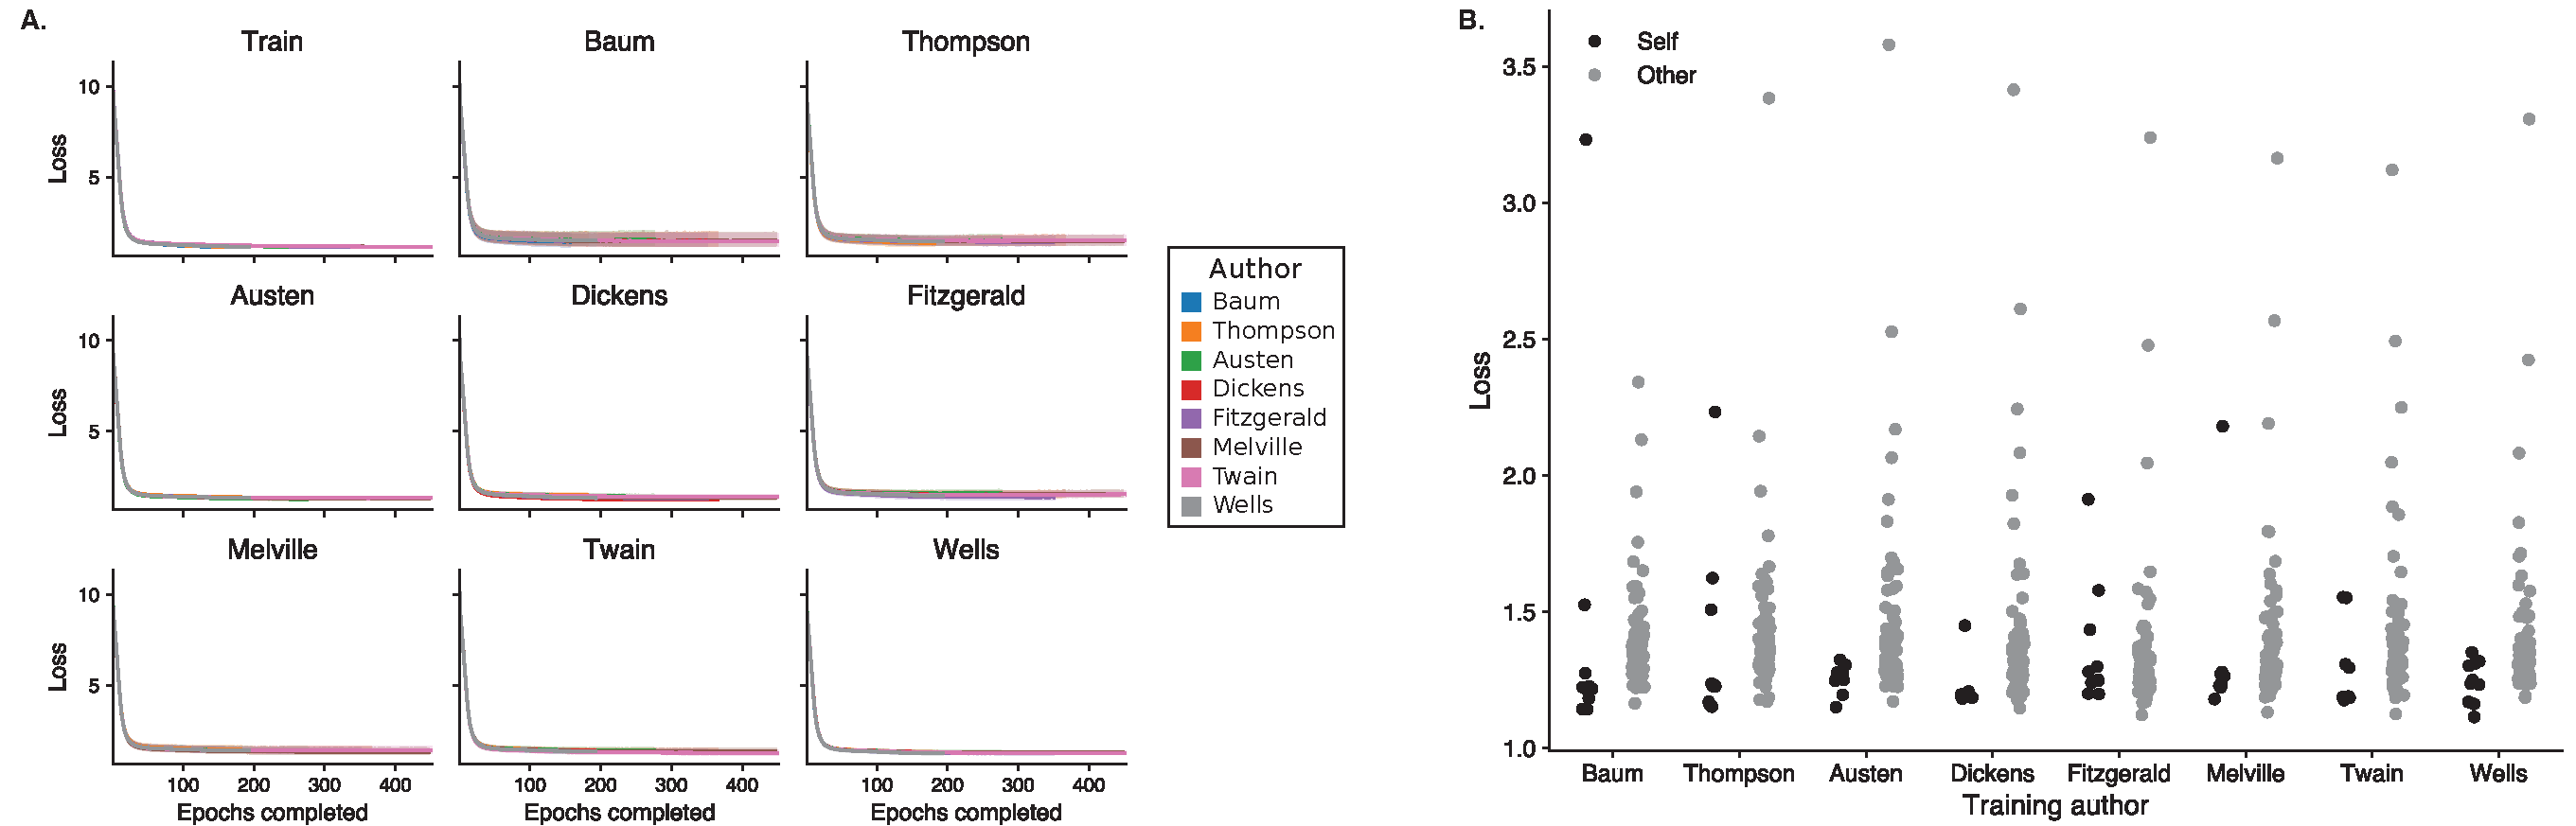
\includegraphics[width=\textwidth]{figs/loss_all_authors_pos.pdf}


  \caption{\textbf{Cross-entropy loss across models and
      authors using only parts of speech.} Follows the general format of Figure~\crossentropy~in the main text,
      but uses models trained on only parts of speech. All words are replaced with their corresponding part of speech tag.
      \textbf{A.} Average cross-entropy loss on
    \textit{Train}ing data and held-out test data from each author,
    plotted as a function of the number of training epochs. Each color
    denotes a model trained on a single author's work.  Error ribbons
    denote bootstrap-estimated 95\% confidence intervals over 10
    random seeds. \textbf{B.} Cross-entropy loss assigned to held-out
    test data by each author's model ($x$-axis). Held-out test data is
    either from the \textit{same} author (black) or from
    \textit{other} authors (gray). Each dot denotes the average loss
    (across all 1024-token chunks) for a single random seed.}
\label{fig:all-losses-pos}
\end{figure*}

\begin{figure*}[h]
  \centering
  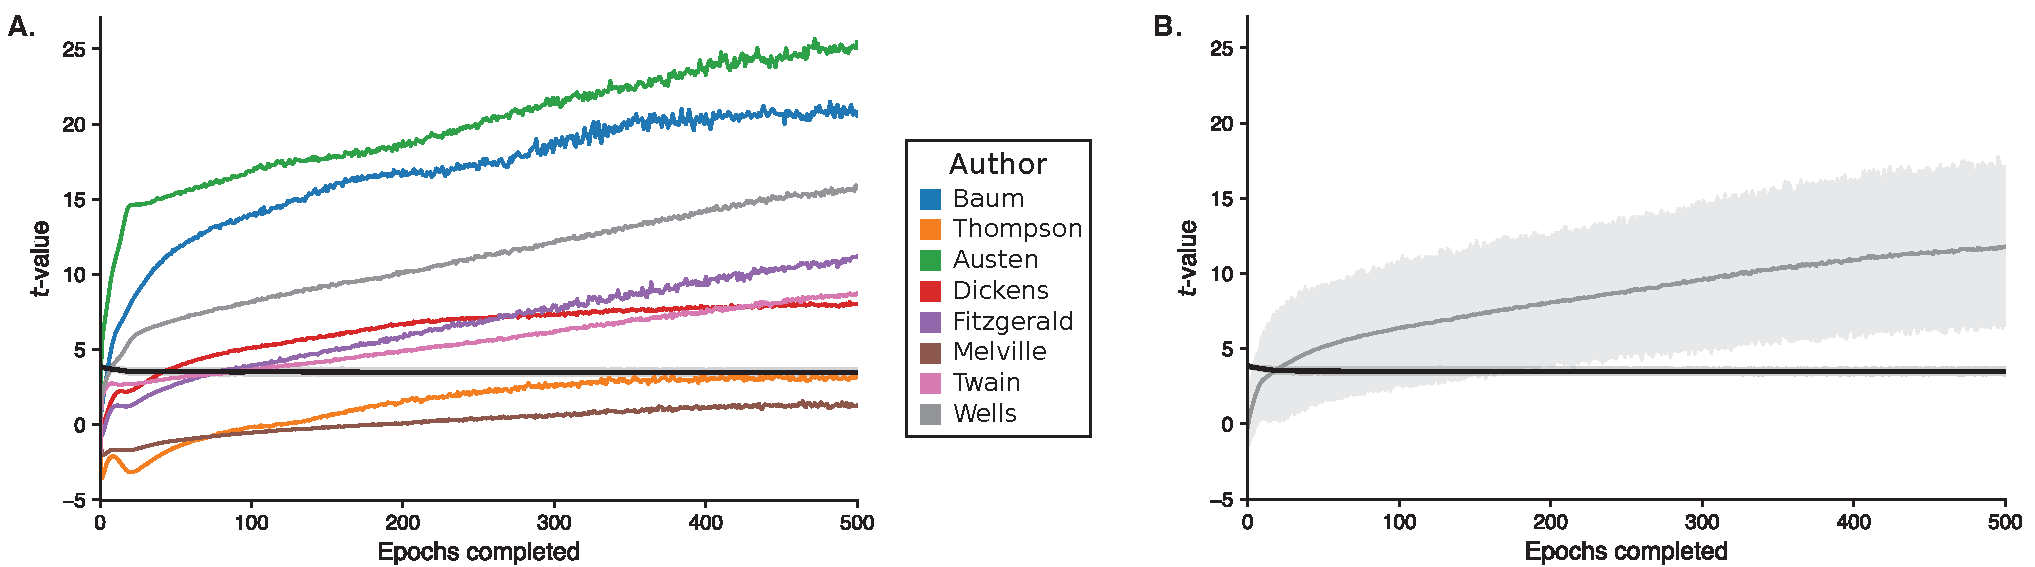
\includegraphics[width=\textwidth]{figs/t_stats_content_only.pdf}


\caption{\textbf{Same vs. other author comparisons, by model, using only
content words.} Follows the general format of Figure~\ttests~in the main text,
but uses models trained on only content words. All function words are masked
out using \texttt{<FUNC>}. \textbf{A.} Each curve denotes, as a function of the
number of training epochs, the the $t$-statistic from a $t$-test comparing the
distribution of losses (across random seeds) assigned to held-out texts from
the given author (color) versus held-out texts from all other authors.
\textbf{B.} The average $t$-statistic across all eight authors, as a function
of the number of training epochs. The black curves in both panels indicates the
average $t$-value corresponding to $p = 0.001$, for each epoch. Error ribbons
denote bootstrap-estimated 95\% confidence intervals across authors.}

\label{fig:t-stats-content}
\end{figure*}

\begin{figure*}[h]
  \centering
  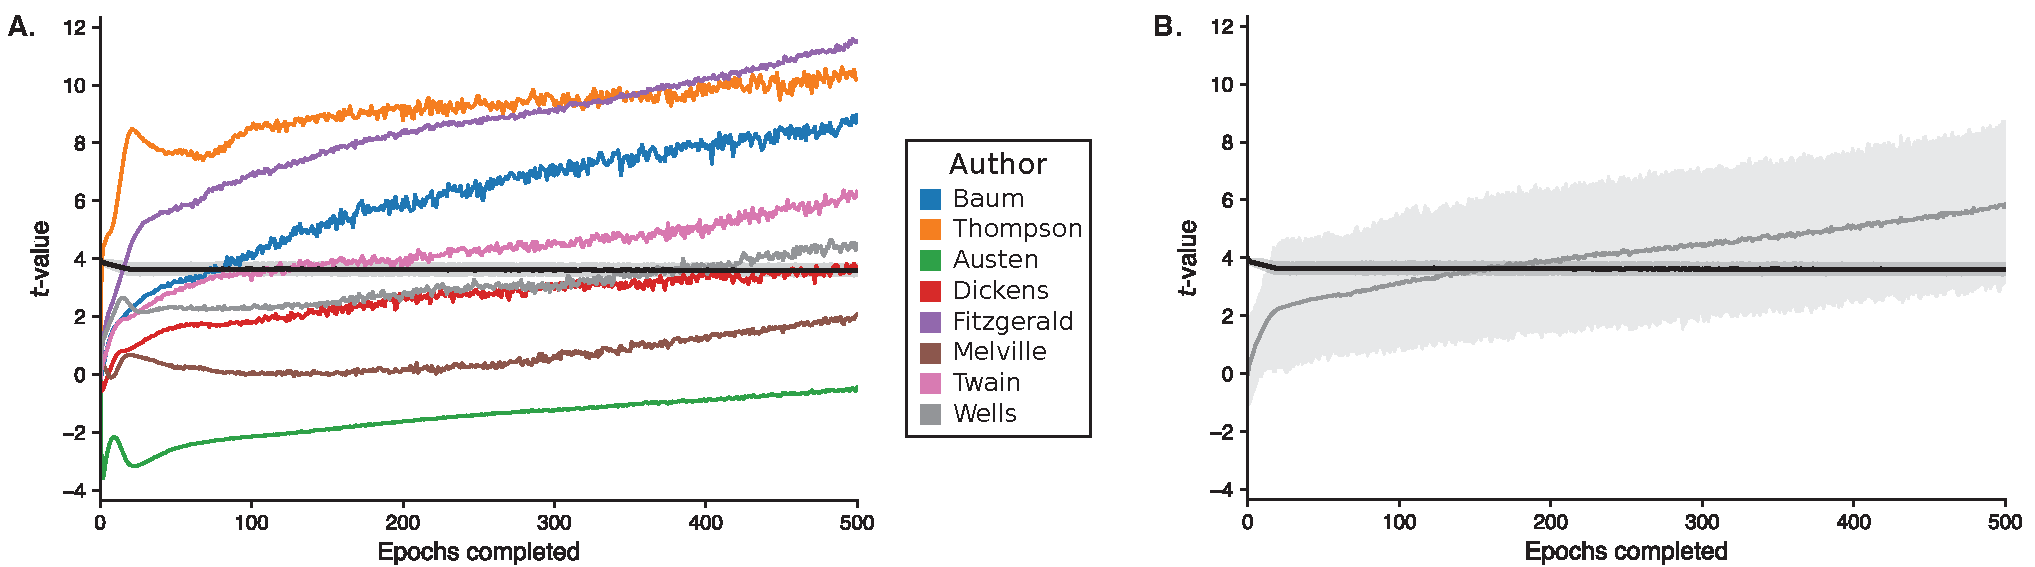
\includegraphics[width=\textwidth]{figs/t_stats_function_only.pdf}


\caption{\textbf{Same vs. other author comparisons, by model, using only
function words.} Follows the general format of Figure~\ttests~in the main text,
but uses models trained on only function words. All content words are masked
out using \texttt{<CONTENT>}. \textbf{A.} Each curve denotes, as a function of
the number of training epochs, the the $t$-statistic from a $t$-test comparing
the distribution of losses (across random seeds) assigned to held-out texts
from the given author (color) versus held-out texts from all other authors.
\textbf{B.} The average $t$-statistic across all eight authors, as a function
of the number of training epochs. The black curves in both panels indicates the
average $t$-value corresponding to $p = 0.001$, for each epoch. Error ribbons
denote bootstrap-estimated 95\% confidence intervals across authors.}

\label{fig:t-stats-function}
\end{figure*}

\begin{figure*}[h]
  \centering
  \DIFdelbeginFL %DIFDELCMD < 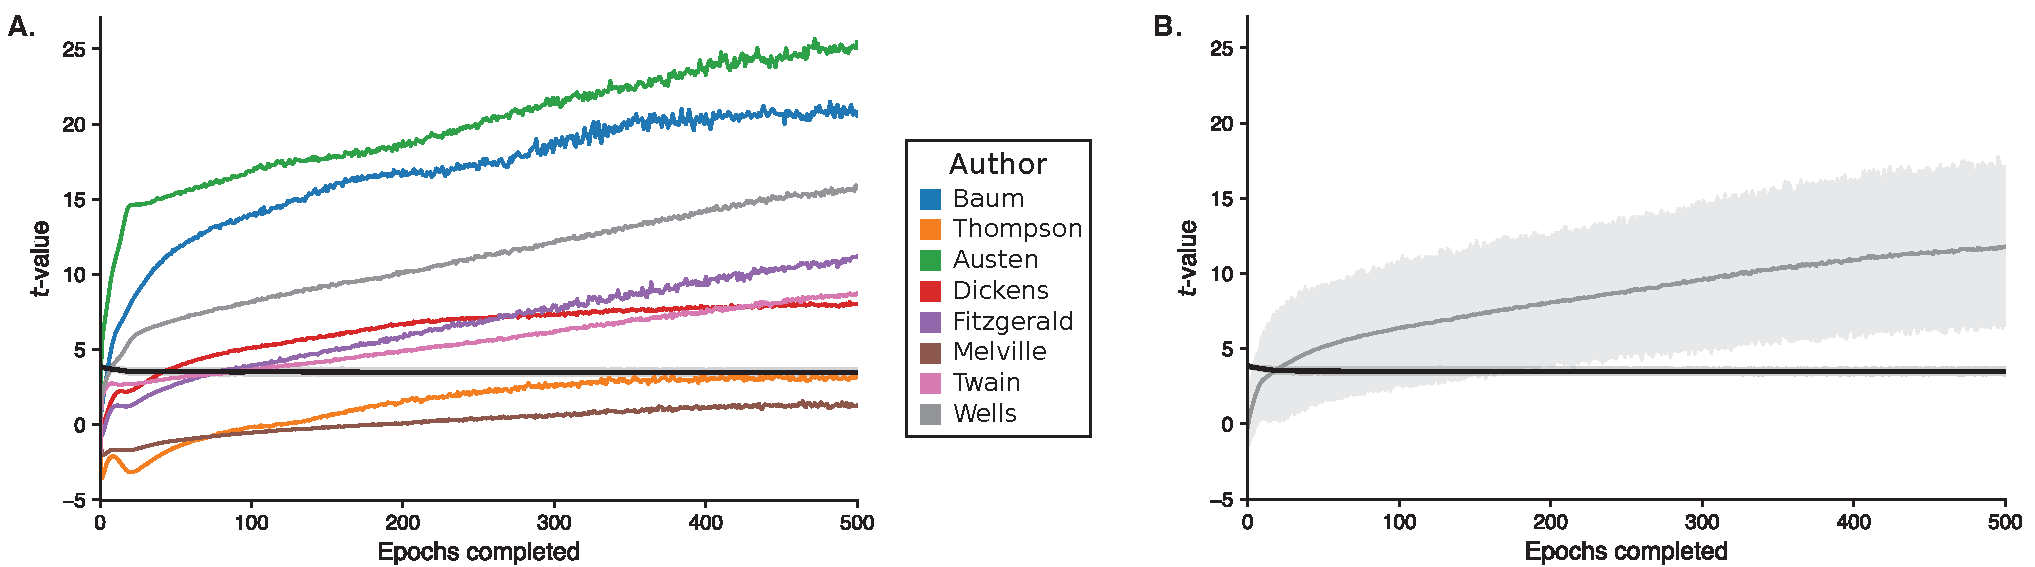
\includegraphics[width=\textwidth]{figs/t_stats_content_only.pdf}
%DIFDELCMD < %%%
\DIFdelendFL \DIFaddbeginFL 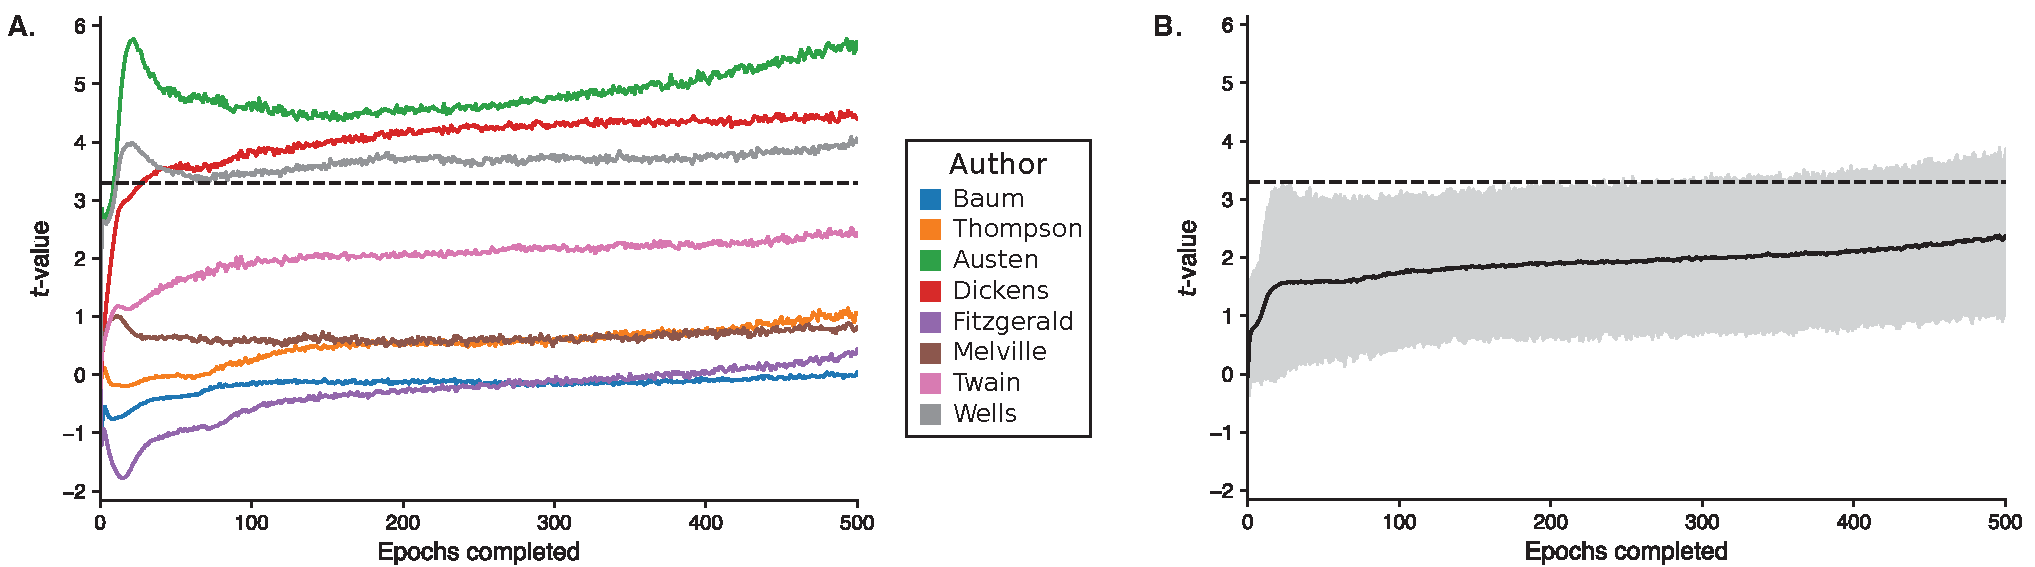
\includegraphics[width=\textwidth]{figs/t_stats_pos.pdf}
\DIFaddendFL 


\caption{\textbf{Same vs. other author comparisons, by model, using only parts
of speech.} Follows the general format of Figure~\ttests~in the main text, but
uses models trained on only parts of speech. All words are replaced with their
corresponding part of speech tag. \textbf{A.} Each curve denotes, as a function
of the number of training epochs, the the $t$-statistic from a $t$-test
comparing the distribution of losses (across random seeds) assigned to held-out
texts from the given author (color) versus held-out texts from all other
authors. \textbf{B.} The average $t$-statistic across all eight authors, as a
function of the number of training epochs. The black curves in both panels
indicates the average $t$-value corresponding to $p = 0.001$, for each epoch.
Error ribbons denote bootstrap-estimated 95\% confidence intervals across
authors.}

\label{fig:t-stats-pos}
\end{figure*}

\begin{figure*}[h]
  \centering
  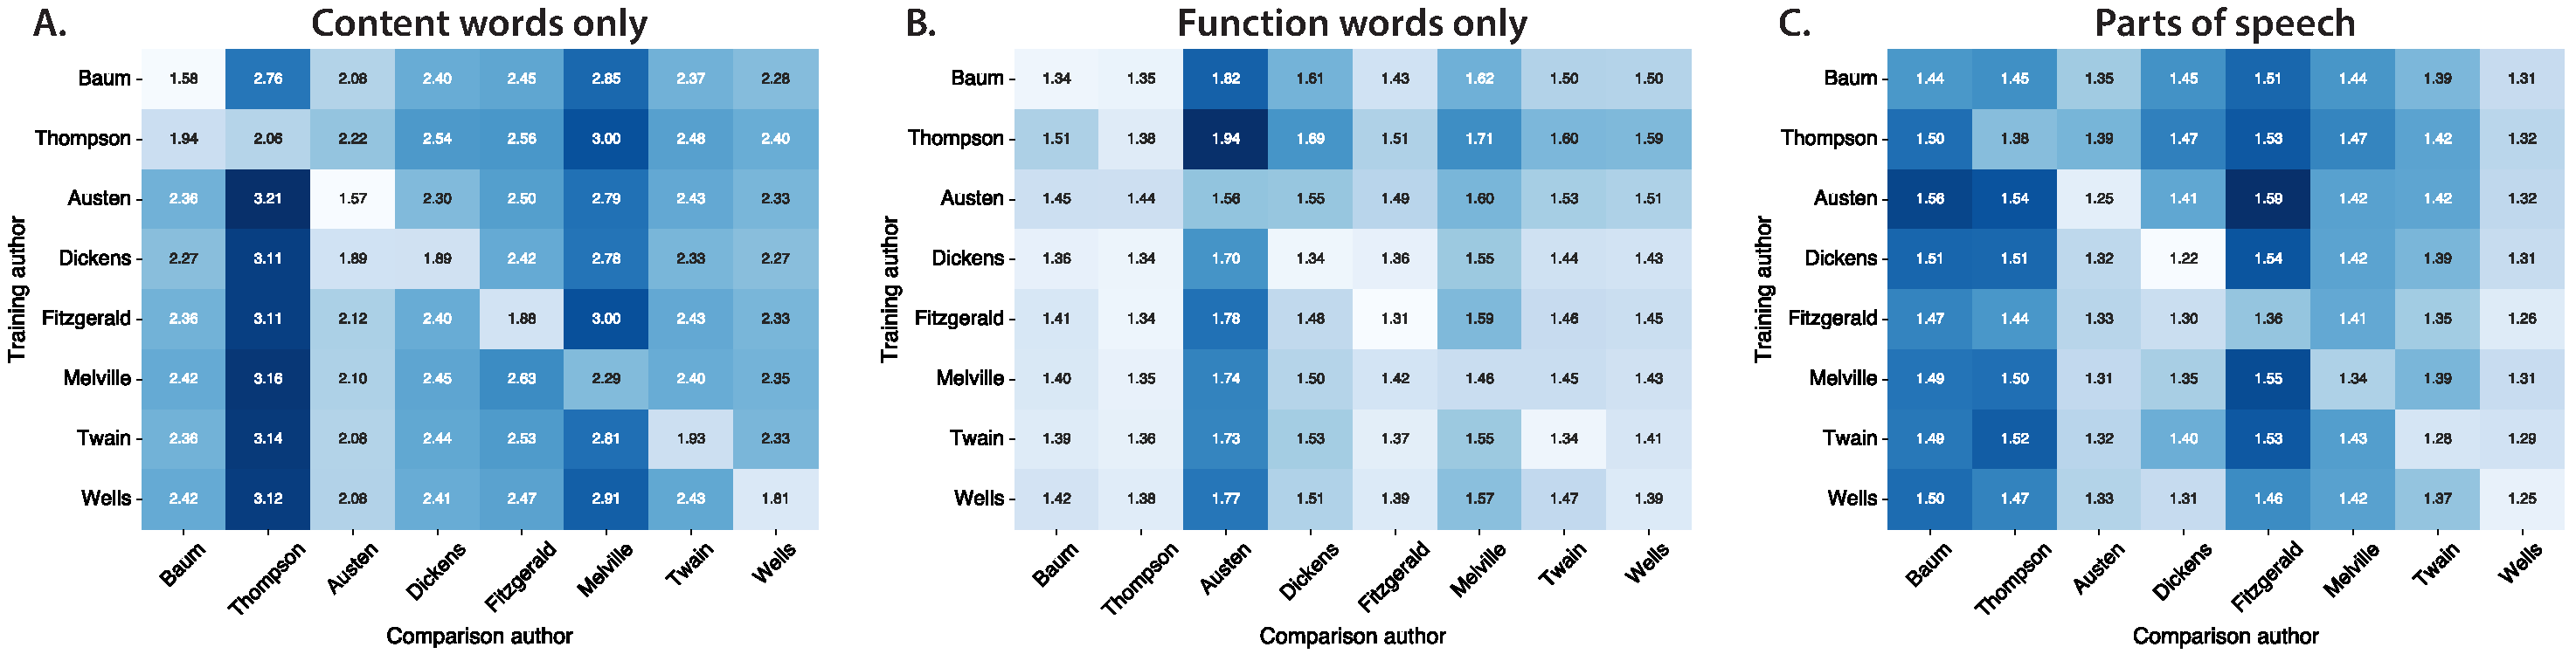
\includegraphics[width=\textwidth]{figs/confustion_matrices_variants.pdf}


\caption{\textbf{Confusion matrices.} Follows the general format of
Figure~\confusion~in the main text, but shows confusion matrices for models
trained on only content words (A), only function words (B), and only parts of
speech (C). Within each panel, the matrix displays the average cross-entropy loss assigned by
models trained on each author's writing (column) to held-out texts from each
author (row), after subtracting the native author's baseline loss.}
\label{fig:confusion-matrix-combined}

\end{figure*}


\begin{figure*}[t]
  \centering
  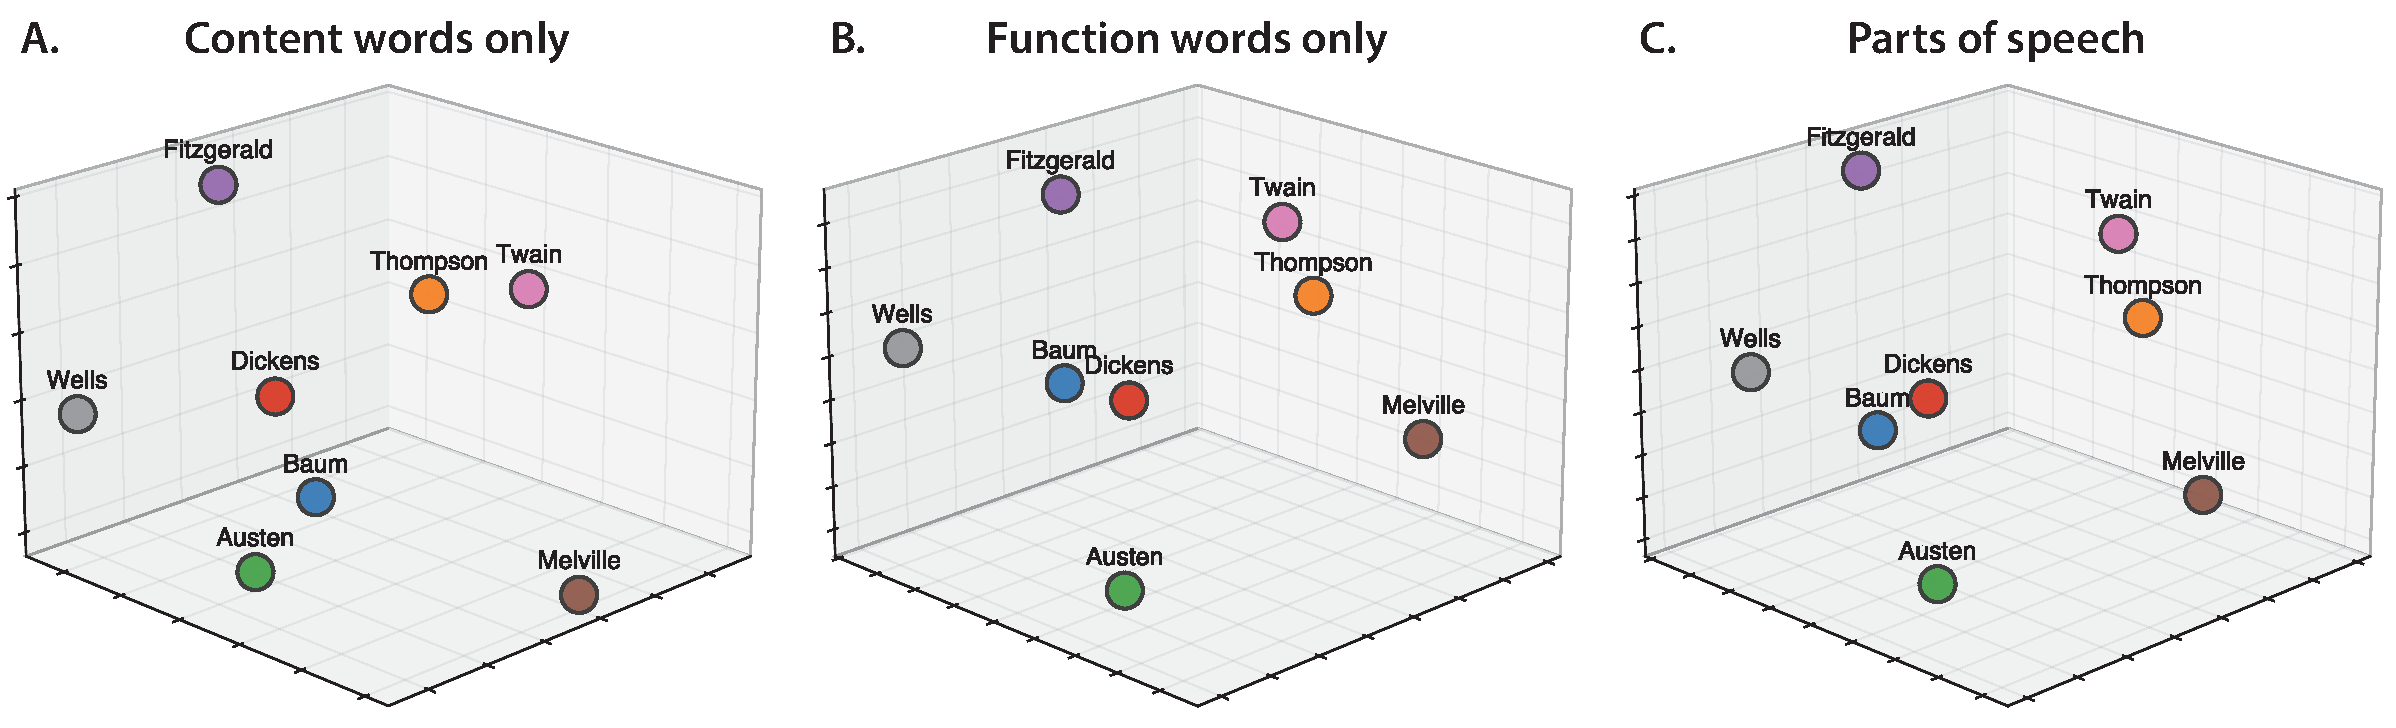
\includegraphics[width=\textwidth]{figs/mds_plots_variants.pdf}


\caption{\textbf{Multidimensional scaling plots.} Follows the general format of
Figure~\mds~in the main text, but shows MDS projections of the (symmetrized)
average cross entropy loss matrices shown in
Figure~\ref{fig:confusion-matrix-combined}, for models trained on only content
words (A), only function words (B), and only parts of speech (C).}
\label{fig:mds} \end{figure*}

\clearpage



\DIFaddbegin \begin{center}
  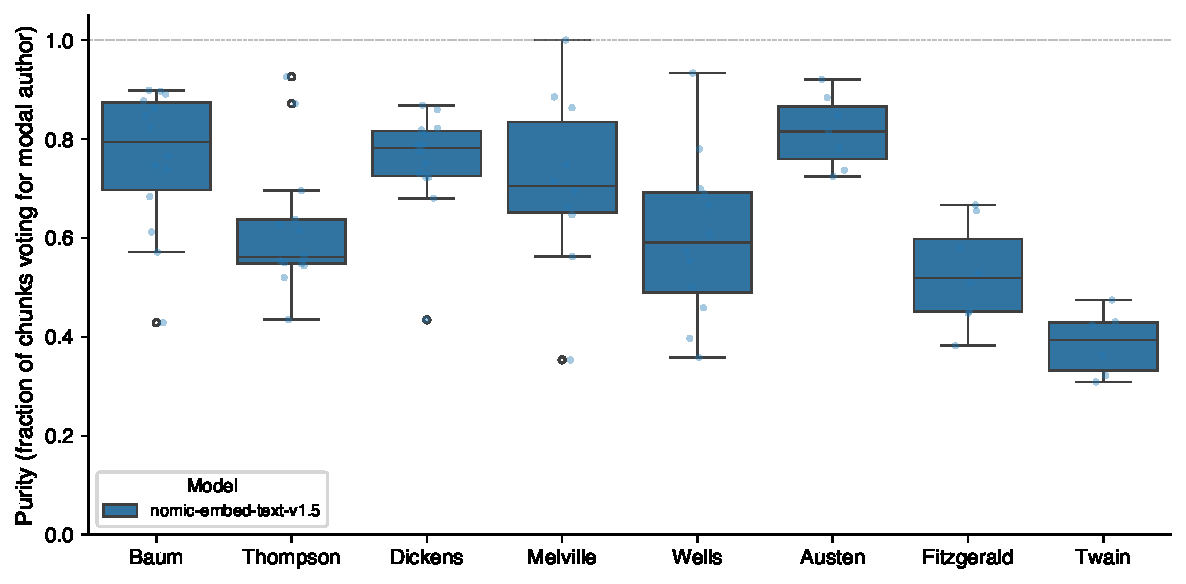
\includegraphics[width=\textwidth]{figs/source/embedding_purity.pdf}
  \captionof{figure}{\textbf{Chunk-level purity for embedding-based attribution.}
  Distribution of purity scores (fraction of chunks voting for the modal
  author) across books, grouped by author and model. Higher purity indicates
  stronger consensus among chunk-level predictions.}
  \label{fig:embedding-purity}
\end{center}

\begin{center}
  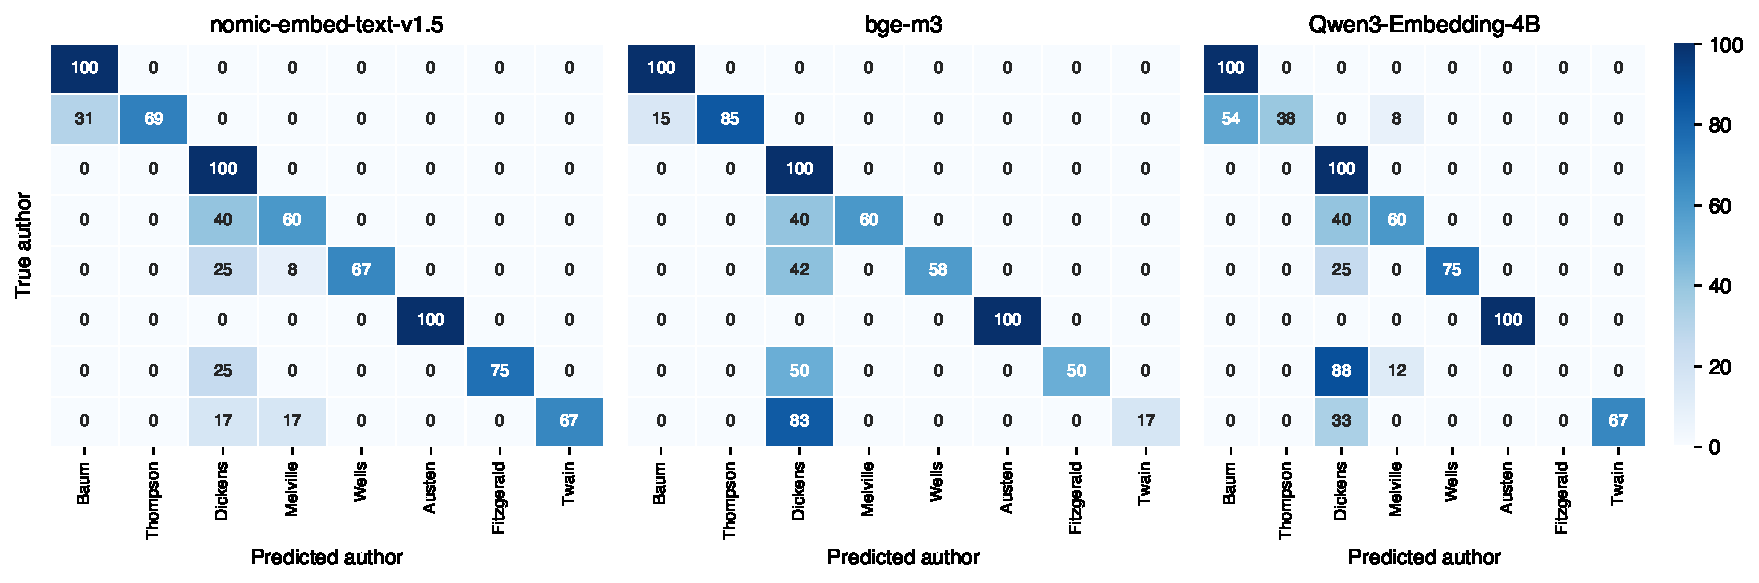
\includegraphics[width=\textwidth]{figs/source/embedding_confusion.pdf}
  \captionof{figure}{\textbf{Confusion matrices for embedding-based attribution.}
  Each panel shows the percentage of books by each true author (rows) that
  were classified as each predicted author (columns). Diagonal entries
  represent correct attributions.}
  \label{fig:embedding-confusion}
\end{center}

\clearpage

\DIFaddend \begin{table}[h]
\centering
\small
\begin{tabular}{lccc}
\hline
\textbf{Model} & \textbf{$t$-stat} & \textbf{df} & \textbf{$p$-value}\\
\hline
Baum         & 20.58 & 68.36 & $5.27 \times 10^{-31}$  \\
Thompson     & 3.29 & 11.33 & $6.97 \times 10^{-3}$  \\
Austen       & 25.46 & 70.33 & $3.20 \times 10^{-37}$  \\
Dickens      & 8.04 & 37.39 & $1.13 \times 10^{-9}$  \\
Fitzgerald   & 11.21 & 49.02 & $3.97 \times 10^{-15}$  \\
Melville     & 1.28 & 10.28 & $0.2274$  \\
Twain        & 8.73 & 22.50 & $1.12 \times 10^{-8}$  \\
Wells        & 15.79 & 71.87 & $4.53 \times 10^{-25}$  \\
\hline
\end{tabular}

\caption{\textbf{Loss differences between same-author and other-author texts
using only content words.} Follows the general format of Table~\authortable~in
the main text, but uses models trained on only content words. Each row displays
the results of a $t$-test comparing the average loss values assigned by each
author's model (after training is complete) to the author's held-out text and
to the other authors' randomly sampled texts.}

\label{tab:t-tests-content}
\end{table}

\begin{table}[h]
\centering
\small
\begin{tabular}{lccc}
\hline
\textbf{Model} & \textbf{$t$-stat} & \textbf{df} & \textbf{$p$-value}\\
\hline
Baum         & 8.97 & 20.85 & $1.34 \times 10^{-8}$  \\
Thompson     & 10.20 & 22.96 & $5.39 \times 10^{-10}$  \\
Austen       & -0.46 & 9.52 & $0.6581$  \\
Dickens      & 3.69 & 17.46 & $1.73 \times 10^{-3}$  \\
Fitzgerald   & 11.52 & 77.98 & $1.70 \times 10^{-18}$  \\
Melville     & 2.08 & 17.29 & $0.0529$  \\
Twain        & 6.31 & 34.66 & $3.14 \times 10^{-7}$  \\
Wells        & 4.49 & 15.94 & $3.76 \times 10^{-4}$  \\
\hline
\end{tabular}

\caption{\textbf{Loss differences between same-author and other-author texts
using only function words.} Follows the general format of Table~\authortable~in
the main text, but uses models trained on only function words. Each row displays
the results of a $t$-test comparing the average loss values assigned by each
author's model (after training is complete) to the author's held-out text and
to the other authors' randomly sampled texts.}

\label{tab:t-tests-function}
\end{table}

\begin{table}[h]
\centering
\small
\begin{tabular}{lccc}
\hline
\textbf{Model} & \textbf{$t$-stat} & \textbf{df} & \textbf{$p$-value}\\
\hline
Baum         & 0.04 & 9.22 & $0.9695$  \\
Thompson     & 1.05 & 10.91 & $0.3179$  \\
Austen       & 5.72 & 77.97 & $1.89 \times 10^{-7}$  \\
Dickens      & 4.41 & 62.85 & $4.14 \times 10^{-5}$  \\
Fitzgerald   & 0.43 & 14.25 & $0.6704$  \\
Melville     & 0.81 & 11.98 & $0.4337$  \\
Twain        & 2.43 & 20.88 & $0.0240$  \\
Wells        & 4.05 & 56.90 & $1.55 \times 10^{-4}$  \\
\hline
\end{tabular}

\caption{\textbf{Loss differences between same-author and other-author texts
using only parts of speech.} Follows the general format of Table~\authortable~in
the main text, but uses models trained on only parts of speech. Each row displays
the results of a $t$-test comparing the average loss values assigned by each
author's model (after training is complete) to the author's held-out text and
to the other authors' randomly sampled texts.}

\label{tab:t-tests-pos}
\DIFaddbeginFL \end{table}

\begin{table}[h]
\centering
\begin{tabular}{lccc}
\toprule
\textbf{\DIFaddFL{Model}} & \textbf{\DIFaddFL{Parameters}} & \textbf{\DIFaddFL{Book accuracy}} & \textbf{\DIFaddFL{Avg.\ purity}} \\
\midrule
\DIFaddFL{nomic-embed-text-v1.5 }& \DIFaddFL{137M }& \DIFaddFL{81.0\% (68/84) }& \DIFaddFL{0.666 }\\
\DIFaddFL{bge-m3 }& \DIFaddFL{568M }& \DIFaddFL{76.2\% (64/84) }& \DIFaddFL{0.694 }\\
\DIFaddFL{Qwen3-Embedding-4B }& \DIFaddFL{4.0B }& \DIFaddFL{70.2\% (59/84) }& \DIFaddFL{0.703 }\\
\midrule
\DIFaddFL{Predictive comparison (ours) }& \DIFaddFL{0.8M $\times$ 8 }& \DIFaddFL{100\% (84/84) }& \DIFaddFL{--- }\\
\bottomrule
\end{tabular}
\caption{\textbf{\DIFaddFL{Book-level attribution accuracy for embedding-based
nearest-neighbor classification versus our predictive comparison approach.}}
\DIFaddFL{Purity denotes the fraction of held-out chunks assigned to the modal
(predicted) author. Our approach trains one small GPT-2 model per author from
scratch; embedding methods use a single pre-trained model for all authors.}}
\label{tab:embedding-comparison}
\DIFaddendFL \end{table}


\end{document}
